%% MNRAS LaTeX template
%% Requires mnras.cls — available from MNRAS author guide or CTAN
\documentclass[a4paper,fleqn,usenatbib]{mnras}

\usepackage{graphicx}
\usepackage{amsmath}
\usepackage{amssymb}
\usepackage{booktabs}
\usepackage{hyperref}

%%--------------------------------------------------------------------
%% Title, authors, affiliations
%%--------------------------------------------------------------------
\title[Pushforward Sensitivity by Perturbation Axis]{%
  Decomposition of Pushforward Sensitivity by Perturbation Axis
  in Galactic Center Orbit Inference}

\author[M. Blumhardt]{%
  Michael Blumhardt$^{1}$\thanks{E-mail: placeholder@institution.edu}
  \\
  $^{1}$[Institution]
}

\date{Accepted 2026 --. Received 2026 --; in original form 2026 --}

\pubyear{2026}

%%--------------------------------------------------------------------
\begin{document}
\label{firstpage}
\pagerange{\pageref{firstpage}--\pageref{lastpage}}
\maketitle

%%--------------------------------------------------------------------
\begin{abstract}
Derived quantities in astrophysical inference pipelines are often treated as
stable summaries of posterior structure, yet sensitivity to underlying
perturbations is rarely characterized in a controlled manner. In Galactic
Center orbit inference, periapsis velocity is a nonlinear function of orbital
parameters and is routinely used in downstream physical interpretation. A
preregistered, deterministic perturbation audit evaluates sensitivity of this
derived quantity under two orthogonal perturbation axes applied to a weighted
empirical posterior: weight perturbations at fixed support and support
perturbations of eccentricity at fixed empirical measure.

Both perturbation classes use an identical rank-structured basis and are
evaluated with the same weighted Wasserstein-1 ($W_1$) metric, isolating the
perturbation axis as the sole structural difference. Weight perturbations
produce linear scaling of $W_1$ and approximately uniform localization of
divergence across the velocity distribution. In contrast, support perturbations
produce super-linear scaling ($W_1(0.090)/W_1(0.010) = 13.92$) and strong
upper-tail concentration, with the top decile contributing 52--71\% of total
divergence. Localization is computed using fixed baseline thresholds, ensuring
invariance to perturbation-induced support expansion.

All perturbations, thresholds, and evaluation criteria were preregistered and
executed without deviation. Results establish that sensitivity of derived
quantities can differ qualitatively by perturbation axis, even under identical
perturbation structure and evaluation. This finding has direct
implications for robustness assessment of orbit inference pipelines and other
astrophysical analyses involving nonlinear transformations of posterior
distributions.
\end{abstract}

\begin{keywords}
methods: statistical -- methods: data analysis -- Galaxy: centre --
stars: kinematics and dynamics
\end{keywords}

%%--------------------------------------------------------------------
\section{Introduction}
\label{sec:intro}

Inference pipelines in astrophysics frequently map posterior distributions
over model parameters to derived physical quantities used for interpretation
and downstream analysis. In Galactic Center orbit studies, posterior samples
over orbital elements are transformed into quantities such as periapsis
velocity, which are then used to assess dynamical constraints and relativistic
effects. These transformations are nonlinear, and sensitivity of derived
quantities to perturbations in the underlying posterior is typically assessed
only through aggregate uncertainty summaries.

Aggregate summaries do not distinguish between structural sources of
sensitivity. In particular, changes in posterior weights and changes in the
support of the distribution represent distinct perturbation modes that
propagate differently through nonlinear transformations. Without controlled
perturbation, these effects are confounded and stability of derived quantities
cannot be attributed to specific mechanisms.

A controlled perturbation framework is introduced to isolate these modes. A
weighted empirical posterior from Galactic Center orbit inference is subjected
to two preregistered perturbation classes: weight perturbations at fixed
support and support perturbations of eccentricity at fixed empirical measure.
Both perturbations use an identical rank-based structure, ensuring that
observed differences arise from the perturbation axis rather than from the
perturbation basis or numerical procedure. Sensitivity is quantified using the
weighted Wasserstein-1 distance between pushforward distributions of periapsis
velocity.

The resulting comparison reveals qualitatively distinct regimes. Weight
perturbations produce linear scaling of divergence and approximately uniform
contributions across the velocity distribution. Support perturbations produce
super-linear scaling and strong concentration of divergence in the
high-velocity tail. Localization is computed using fixed baseline thresholds
derived from the unperturbed distribution, preventing perturbation-dependent
rebinning artifacts.

The objective of this study is not to establish general laws of sensitivity,
but to demonstrate, within a realistic inference pipeline, that pushforward
behavior depends critically on the perturbation axis. This has direct
implications for robustness assessment in orbit inference and more broadly for
astrophysical analyses involving nonlinear transformations of posterior
distributions.

%%--------------------------------------------------------------------
\section{Related work}
\label{sec:relwork}

Stability and sensitivity of Bayesian posteriors have been studied extensively
in the context of inverse problems and uncertainty quantification. Prior work
has established conditions under which posterior distributions exhibit
continuity or Lipschitz stability under perturbations of priors, likelihoods,
or data, often measured in total variation, Hellinger, or Wasserstein distance
\citep{Stuart2010,Sprungk2020}. These results formalize robustness at the level
of the posterior distribution but typically do not address how such
perturbations propagate through nonlinear transformations to derived quantities.

Pushforward measures provide the natural framework for analyzing transformed
distributions, and Wasserstein distances have been used to compare such
measures under deterministic mappings \citep{Villani2009,Santambrogio2015}.
Existing work characterizes continuity properties of pushforward distributions
and establishes bounds on their sensitivity under perturbations of the input
measure. However, these analyses generally treat perturbations in aggregate
and do not distinguish between structurally different classes of perturbation.

In astrophysics, uncertainty propagation through nonlinear inference pipelines
is widely recognized as an important practical issue, particularly in contexts
where derived quantities depend sensitively on underlying parameters
\citep{Do2019}. Prior studies have examined how observational and model
uncertainties propagate through such pipelines, but systematic characterization
of sensitivity structure at the level of transformed posterior distributions
remains limited.

The present study builds on these foundations by introducing a controlled
perturbation framework that isolates weight and support perturbations under a
shared basis, enabling empirical characterization of axis-dependent pushforward
sensitivity within an astrophysical inference pipeline.

%%--------------------------------------------------------------------
\section{Data and baseline construction}
\label{sec:data}

The analysis uses a weighted empirical posterior from Galactic Center orbit
inference \citep{Do2019}. Posterior samples provide values of orbital
parameters including eccentricity and gravitational parameter $GM$, together
with associated weights.

Periapsis velocity is computed deterministically from orbital parameters:
\begin{equation}
  v_p = \sqrt{\frac{GM(1+e)}{a(1-e)}},
  \label{eq:vp}
\end{equation}
where the semi-major axis $a$ is derived from the orbital period and
gravitational parameter. All transformations are deterministic and applied once
to construct the baseline pushforward distribution.

Baseline statistics are computed using weighted empirical measures. No
resampling or stochastic approximation is used.

%%--------------------------------------------------------------------
\section{Perturbation framework}
\label{sec:framework}

\subsection{Rank-based perturbation basis}
\label{sec:rankbasis}

A rank-based score is constructed from ascending order of eccentricity:
\begin{equation}
  f_i = \frac{r_i - (N+1)/2}{(N-1)/2},
  \label{eq:fi}
\end{equation}
where $r_i$ is the stable ascending rank of $e_i$. This score defines a
deterministic perturbation direction that is symmetric and bounded in
$[-1, 1]$.

\subsection{Weight perturbation}
\label{sec:weightpert}

Weight perturbations are applied at fixed support:
\begin{equation}
  w_i(\varepsilon) \propto w_i(1 + \varepsilon f_i),
  \label{eq:wpert}
\end{equation}
with normalization applied after perturbation. Support points remain
unchanged. The perturbation amplitude grid is
$\varepsilon \in \{0.00, 0.01, 0.05, 0.10\}$.

\subsection{Support perturbation}
\label{sec:supppert}

Support perturbations are applied to eccentricity at fixed weights:
\begin{equation}
  \tilde{e}_i(\delta) = e_i + \delta f_i.
  \label{eq:epert}
\end{equation}
Weights remain fixed. The perturbation is applied deterministically to each
sample; no resampling or stochastic modification of support is performed.
Domain constraints $0 < \tilde{e}_i < 1$ are enforced for all samples at all
$\delta$. The perturbation amplitude grid is
$\delta \in \{0.000, 0.010, 0.050, 0.090\}$, with grid maximum set below a
preregistered domain ceiling ($0.090 < 0.097$).

\subsection{Axis isolation}
\label{sec:isolation}

Both perturbation classes use the same rank-based basis $f_i$ and identical
$W_1$ estimation. The perturbation axis (weights versus support) is therefore
the only structural difference between conditions.

%%--------------------------------------------------------------------
\section{Metrics}
\label{sec:metrics}

\subsection{Weighted Wasserstein-1 distance}
\label{sec:w1}

Sensitivity is quantified using weighted $W_1$ distance between pushforward
distributions. The algorithm follows a discrete-measure formulation:
duplicate-support aggregation by exact floating-point key equality, sorted
union support, sequential CDF accumulation, and interval integration of
absolute CDF differences. This corresponds to the 1-Wasserstein distance
between discrete weighted measures under the $L^1$ ground metric, evaluated
exactly via cumulative distribution functions on the union support. No library
implementation is used. The same implementation is applied identically to both
perturbation axes.

\subsection{Localization}
\label{sec:localization}

Localization is quantified using decile contributions to total $W_1$. The
support is partitioned into ten equal-probability bins defined by quantiles of
the baseline distribution. The per-decile $W_1$ contribution is the sum of
$|F_0(x) - F_\delta(x)|\,\Delta x$ over all intervals whose left endpoint
falls within that bin.

Decile thresholds are computed once from the baseline distribution and held
fixed across all perturbations. This ensures that localization differences are
not induced by perturbation-dependent rebinning.

%%--------------------------------------------------------------------
\section{Results}
\label{sec:results}

\subsection{Weight perturbation}
\label{sec:res_weight}

Weight perturbations produce linear scaling of $W_1$ with perturbation
amplitude. The ratio $W_1(0.10)/W_1(0.01) = 9.95$ matches the amplitude ratio
of 10, confirming linear response to within numerical precision.

Decile contributions are approximately uniform, ranging from 9.1\% to 10.7\%
across all ten bins (Table~\ref{tab:contrast}, Fig.~\ref{fig:localization}
left). The distribution of localization fractions is invariant across
perturbation amplitude: fractions at $\varepsilon = 0.01$, $0.05$, and $0.10$
are identical to three decimal places. This invariance is the signature of a
coherent, globally distributed deformation of the cumulative distribution.

\subsection{Support perturbation}
\label{sec:res_support}

Support perturbations produce super-linear scaling of $W_1$. The ratio
$W_1(0.090)/W_1(0.010) = 13.92$ substantially exceeds the linear prediction
of 9 (Fig.~\ref{fig:scaling} right).

Decile contributions are strongly concentrated in the top decile, which
accounts for 52\% of total $W_1$ at $\delta = 0.010$, rising to 71\% at
$\delta = 0.090$ (Fig.~\ref{fig:localization} right). The remaining nine
deciles collectively contribute less than 30\% of total divergence. This
concentration intensifies with perturbation amplitude, reflecting progressive
amplification at high eccentricity where $v_p(e)$ is most sensitive.

A secondary contribution of 27--33\% is observed in the lowest decile. This
reflects asymmetric transport under the rank-based perturbation, which shifts
low-eccentricity samples toward lower $v_p$. The dominant feature of the
localization pattern remains upper-tail concentration.

In Fig.~\ref{fig:scaling}, the support-perturbation curve departs
systematically above the linear reference, in contrast to the
weight-perturbation curve, which lies on the reference line across all
amplitudes.

\subsection{Regime contrast}
\label{sec:contrast}

The two perturbation axes produce qualitatively distinct regimes under the
same basis and evaluation metric (Table~\ref{tab:contrast}).

\begin{table}
  \centering
  \caption{Regime contrast between perturbation axes.}
  \label{tab:contrast}
  \resizebox{\columnwidth}{!}{%
  \begin{tabular}{l l l}
    \toprule
    Quantity & Weight axis & Support axis \\
    \midrule
    $W_1$ scaling        & Linear ($\times$10.0 per decade) & Super-linear ($\times$13.9) \\
    D10 fraction         & $\approx 0.107$                  & $0.525$--$0.710$            \\
    D1 fraction          & $\approx 0.091$                  & $0.275$--$0.329$            \\
    Localization         & Broadly distributed              & Upper-tail concentrated     \\
    \bottomrule
  \end{tabular}%
  }
\end{table}

%%--------------------------------------------------------------------
\section{Interpretation}
\label{sec:interpretation}

The observed regime contrast is consistent with nonlinear amplification in the
pushforward map $v_p(e)$, which increases sensitivity near $e \to 1$. Weight
perturbations redistribute mass without altering the nonlinear mapping,
producing linear and broadly distributed effects. Support perturbations move
samples along the nonlinear map, producing amplified and localized effects
proportional to local gradient magnitude.

No analytic derivation is claimed. The mechanism is presented as a consistency
explanation for the observed scaling and localization, supported by the
synthetic demonstration in Appendix~\ref{sec:appendix_a}.

%%--------------------------------------------------------------------
\section{Scope and limitations}
\label{sec:scope}

Results apply to the specific posterior structure used \citep{Do2019}, the
periapsis velocity transformation defined in equation~(\ref{eq:vp}), and the
defined perturbation classes at the specified amplitude grids. No claim is made
regarding universal behavior across all posteriors or transformations,
invariance of the regime contrast under alternative perturbation bases, or
general robustness of derived quantities in other inference pipelines.

%%--------------------------------------------------------------------
\section{Conclusion}
\label{sec:conclusion}

A preregistered perturbation audit demonstrates that pushforward sensitivity
depends qualitatively on perturbation axis. Weight perturbations produce
linear, globally distributed divergence. Support perturbations produce
super-linear, tail-concentrated divergence. This distinction arises under
identical perturbation bases and evaluation metrics, isolating the perturbation
axis as the determining factor.

These findings provide a structured method for diagnosing robustness of derived
quantities in astrophysical inference pipelines and highlight the importance of
distinguishing perturbation modes in sensitivity analysis.

%%--------------------------------------------------------------------
\section*{Data availability}

Preregistered protocols, execution scripts, and results are available at:
Step~3 (weight perturbation): \url{https://osf.io/dmpes};
Step~4 (support perturbation): \url{https://osf.io/fkx46}.
All results in this manuscript can be reproduced deterministically from the
preregistered protocols and released execution artifacts.

%%--------------------------------------------------------------------
\bibliographystyle{mnras}
\bibliography{refs}

%%--------------------------------------------------------------------
%%  FIGURES
%%--------------------------------------------------------------------

\begin{figure*}
  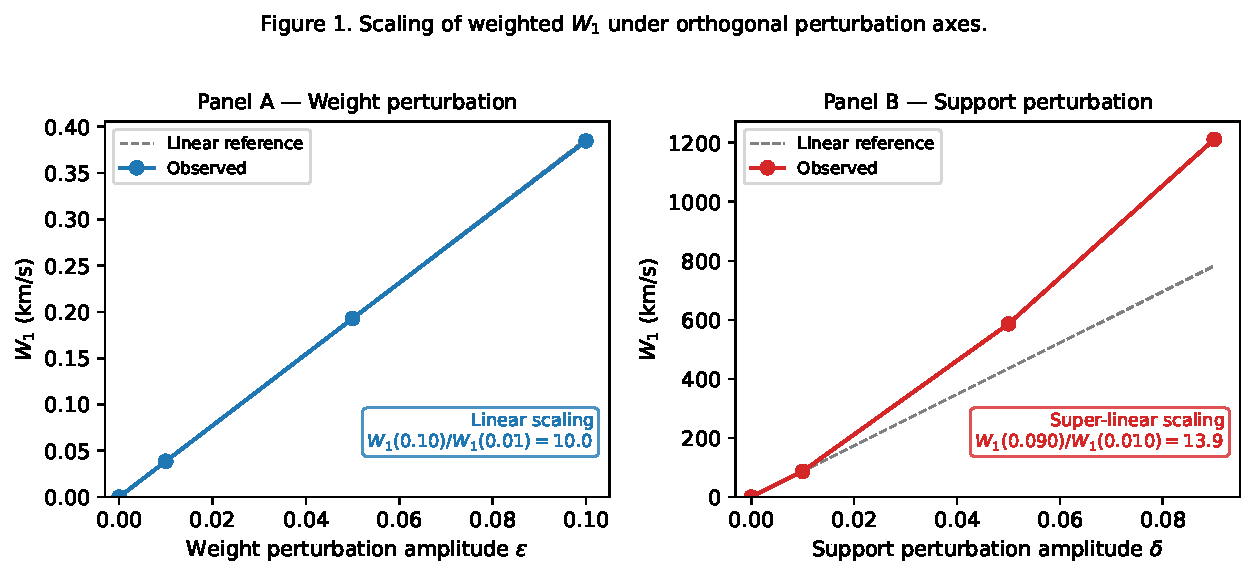
\includegraphics[width=\textwidth]{figure_1_scaling}
  \caption{Scaling of weighted $W_1$ under orthogonal perturbation axes.
    \textit{Left:} weight perturbations at fixed support produce linear
    scaling with perturbation amplitude.
    \textit{Right:} support perturbations at fixed measure produce
    super-linear scaling.
    Dashed lines show linear reference scaling anchored at the smallest
    non-zero perturbation. Both panels use identical rank-based
    perturbation structure; the perturbation axis is the only difference.}
  \label{fig:scaling}
\end{figure*}

\begin{figure*}
  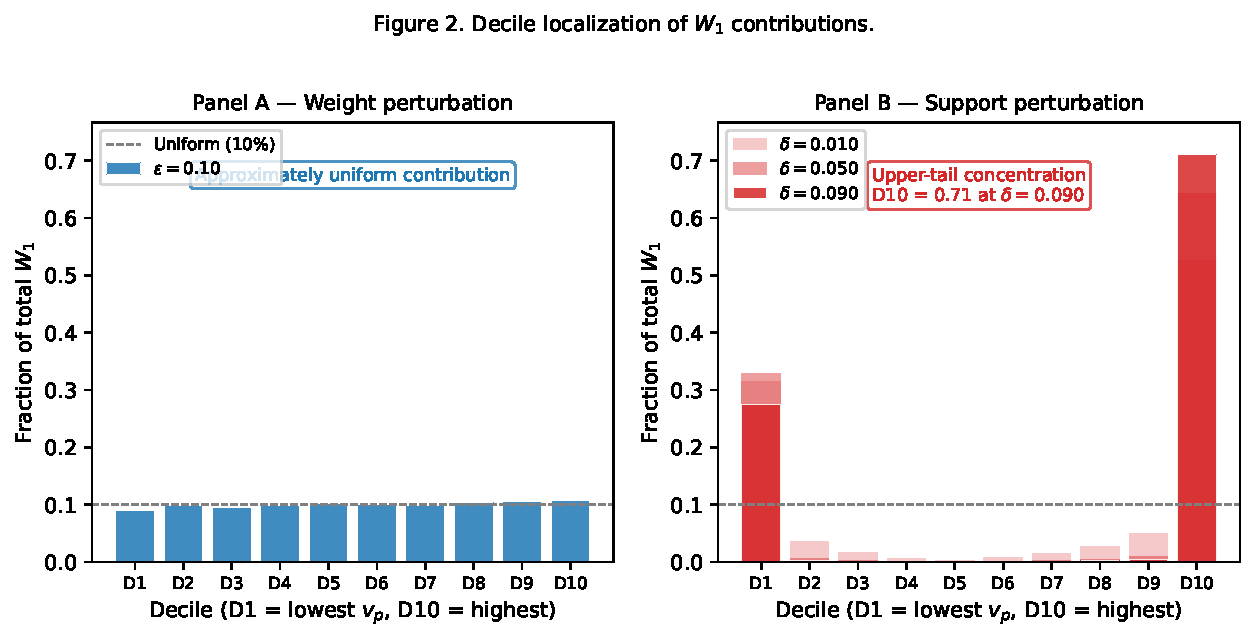
\includegraphics[width=\textwidth]{figure_2_localization}
  \caption{Decile localization of $W_1$ contributions.
    \textit{Left:} weight perturbations produce approximately uniform
    contributions across deciles.
    \textit{Right:} support perturbations concentrate divergence in the
    upper tail, with the top decile contributing the majority of total
    $W_1$.
    Decile thresholds are computed from the baseline distribution and held
    fixed across all perturbations.}
  \label{fig:localization}
\end{figure*}

%%--------------------------------------------------------------------
%%  APPENDIX
%%--------------------------------------------------------------------

\appendix

\section{Minimal synthetic demonstration of axis-dependent pushforward regimes}
\label{sec:appendix_a}

\subsection{Design}

A deterministic grid $e_i \in [0.80, 0.95]$ ($N = 10\,000$) with uniform
weights $w_i = 1/N$ was constructed. The same rank-based perturbation basis
$f_i$ as in the main analysis was applied (equation~\ref{eq:fi}). The
pushforward map was defined as
\begin{equation}
  v(e) = \sqrt{\frac{1+e}{1-e}},
\end{equation}
which preserves the same tail-amplifying nonlinearity as the astrophysical
periapsis-velocity transformation. Weight perturbations at fixed support and
support perturbations at fixed measure were applied using the same axis logic as
in Sections~\ref{sec:weightpert} and~\ref{sec:supppert}. $W_1$ distances were
computed using the same discrete-measure algorithm. Decile localization
thresholds are computed once from the baseline distribution and held fixed
across all perturbations, ensuring that localization differences are not induced
by perturbation-dependent rebinning.

\subsection{Results}

\begin{table}
  \centering
  \caption{Synthetic regime contrast.}
  \label{tab:synthetic}
  \resizebox{\columnwidth}{!}{%
  \begin{tabular}{l l l l}
    \toprule
    Axis & $W_{1,\max}/W_{1,\min+}$ & D10 range & Regime \\
    \midrule
    Weight  & 10.00 & $\approx 0.07$ & linear, broadly distributed \\
    Support & 15.75 & $0.44$--$0.76$ & super-linear, upper-tail concentrated \\
    \bottomrule
  \end{tabular}%
  }
\end{table}

Both perturbation classes use the same rank-based basis $f_i$ and identical
$W_1$ estimation, so the perturbation axis (weights versus support) is the only
structural difference between the two conditions. The weight-axis ratio of 10.00
equals the amplitude ratio, confirming exact linearity. The support-axis ratio
of 15.75 exceeds this by a factor of 1.58, indicating super-linear scaling.

\subsection{Interpretation}

A minimal synthetic weighted empirical system reproduces the same qualitative
contrast observed in the Galactic Center posterior: linear, broadly distributed
response under weight perturbation and super-linear, upper-tail-concentrated
response under support perturbation. Because the synthetic construction removes
dataset-specific posterior structure --- no observational noise, no astrophysical
nuisance parameters, no covariance geometry --- this result is consistent with
the interpretation that the observed regime contrast arises from the geometry of
the pushforward map under nonlinear transformation rather than from idiosyncratic
features of the empirical sample. The synthetic demonstration does not constitute
an independent audited result and is included only as interpretive support for
the structural mechanism identified in the main analysis.

\label{lastpage}
\end{document}
